\documentclass{lug}
\usepackage{graphicx}
\usepackage{amsmath}
\usepackage{bm}
\usepackage{color}

\title{Learning to learn by gradient descent by gradient descent}
\author{Marcin Andrychowicz, Misha Denil, Sergio Gómez Colmenarejo, Matthew W. Hoffman, David Pfau, Tom Schaul, Brendan Shillingfor, Nando de Freitas}
\institute{\textbf{Presented By:} \\ Lou Brand \\ Department of Computer Science\\Colorado School of Mines}
\date{October 31, 2017}

\begin{document}

\section{Motivation}
\frame{
    \frametitle{Description of Gradient Descent}
    \begin{center}
        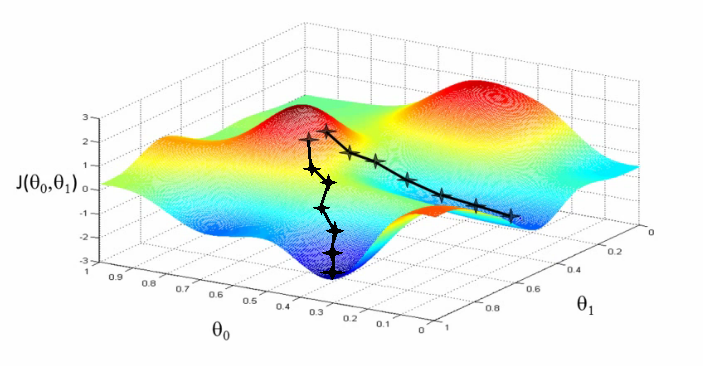
\includegraphics[scale=.6]{images/gradient_descent.png}
    \end{center}
    $$\theta_{t+1} = \theta_t - \alpha_t \nabla f(\theta_t) $$
    \begin{center}
        $J(\theta_t)$ is a function we would like to optimize by varying $\theta_t$
    \end{center}
}

\frame{
    \frametitle{Classic Machine Learning}
    \begin{enumerate}
        \item Prepare Data
        \pause
        \item Design a Model/Function You Want to Minimize
        \pause
        \item Train Model (With an Optimizer!)
        \pause
        \item Use Model
        \pause
    \end{enumerate}
    \textbf{Goal}: Create a framework where we can \textit{learn} how to optimize the function we are interested in minimizing
}

\frame{
    \frametitle{No Free Lunch}
    \pause
    \begin{center}
        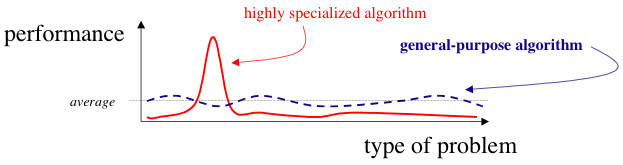
\includegraphics[scale=.5]{images/nfl.png}\\
        Must focus on a subclass of problems.\\
        So let's try and train on a simple example and then add complexity.
    \end{center}
}

\section{Approach}
\frame{
    \frametitle{Learning to Learn}
    \begin{center}
        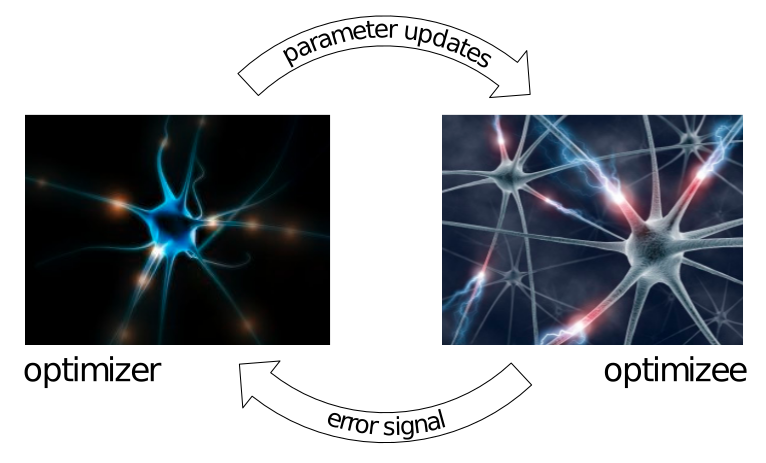
\includegraphics[scale=1]{images/fig1.png}\\
    \end{center}
    \begin{align*}
        \text{Classic Gradient Descent: }
        \theta_{t+1} &= \theta_t - \alpha_t \nabla f(\theta_t) \\
        \text{Learning to Learn: }
        \theta_{t+1} &= \theta_t + g_t(\nabla f(\theta_t), \phi)
    \end{align*}
}

\frame{
    \frametitle{Learning to Learn: Recurrent Neural Network}
    \begin{align*}
        \mathcal{L}(\phi) = \mathbb{E}_f\Big[ \sum^{T}_{t=1} w_t f(\theta_t) \Big] \qquad \text{where} \qquad \theta &= \theta_t + g_t,\\
        \Big[\begin{smallmatrix}g_t \\ h_{t+1}\end{smallmatrix}\Big] &= m(\nabla_t, h_t, \phi)
    \end{align*}
    \begin{center}
        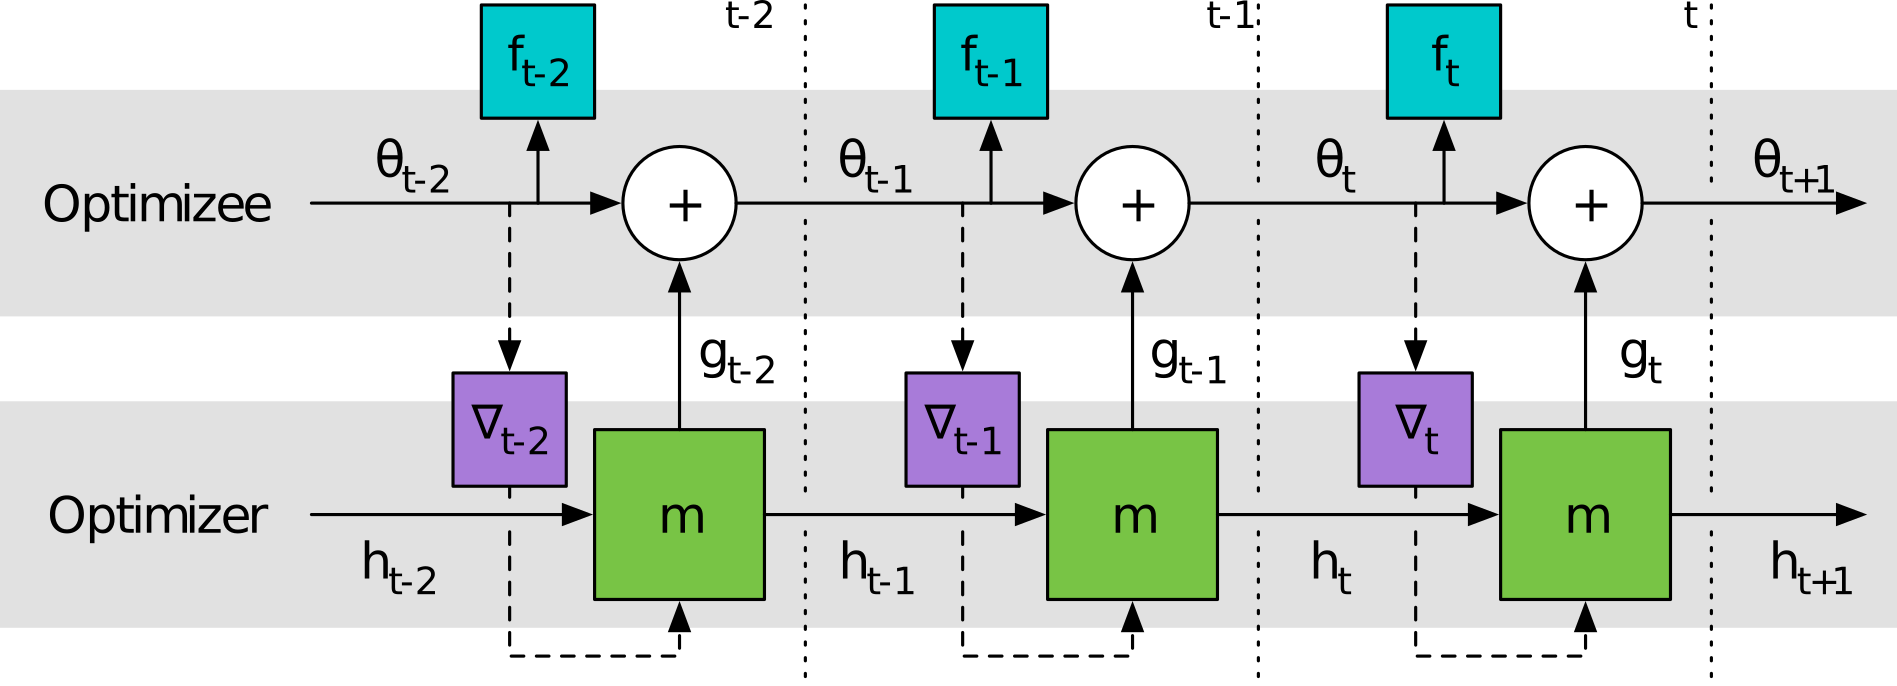
\includegraphics[scale=.7]{images/fig2.png}\\
        \textbf{Note}: Our objective $\mathcal{L}(\phi)$ depends on the entire trajectory of optimization for some horizon $T$
    \end{center}
}

\frame{
    \frametitle{Learning to Learn: Coordinatewise LSTM Optimizer}
    We operate coordinatewise on each $\theta$ to keep the optimizer network small.
    \begin{center}
        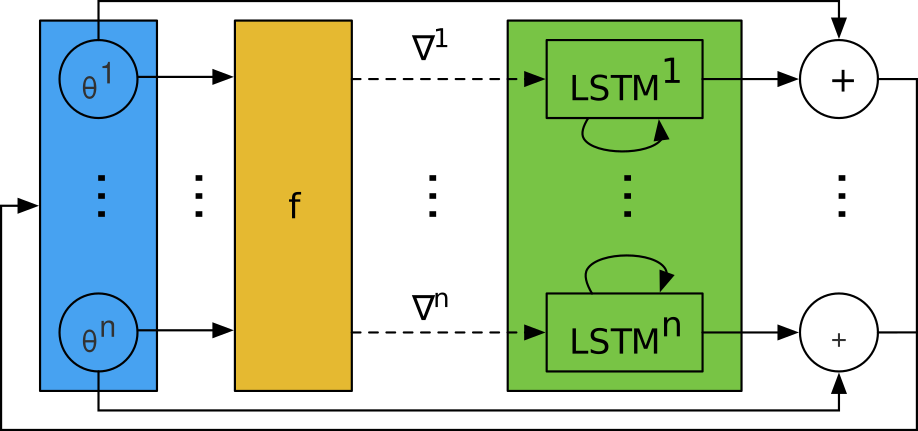
\includegraphics[scale=1]{images/fig3.png}
    \end{center}
    LSTM (a kind of recurrent neural network) allows us to take advangate of the history of updates similar to \textit{momentum} in standard neural networks.
}

\section{Experiments}
\frame{
    \frametitle{Overview}
    \begin{itemize}
        \item In all experiments all trained optimizers use two-layer LSTMs
        \pause
        \item 20 hidden units in each layer
        \pause
        \item Initial minimization is preformed by an ADAM optimizer (training step)
        \pause
        \item Trained optimizer tested against SGD, RMSprop, ADAM, and Nestrov's acclerated gradient (NAG) 
    \end{itemize}
}

\frame{
    \frametitle{Quadratic Functions}
    \begin{center}
        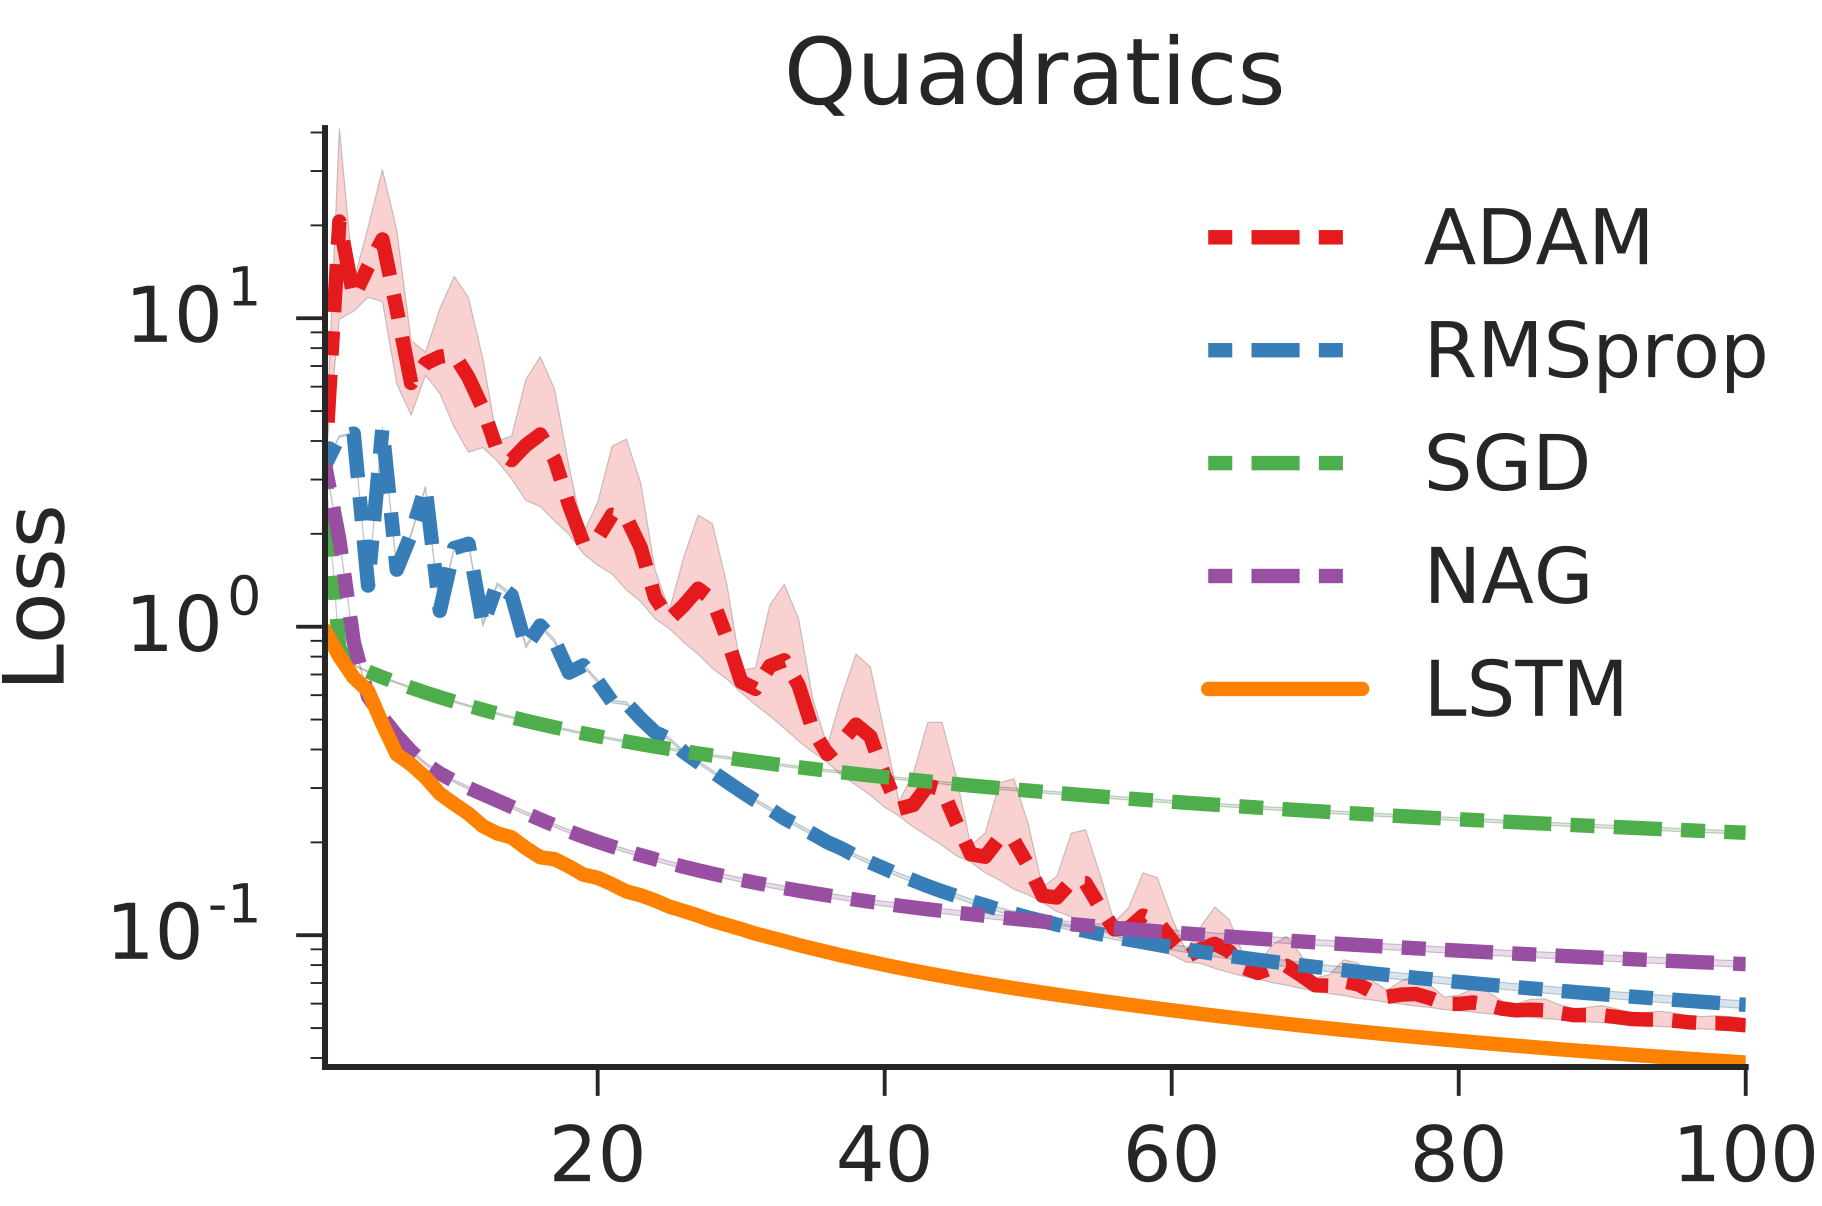
\includegraphics[scale=2]{images/quadratics.png}\\
        Optimize: $f(\theta) = \lVert W\theta - y \rVert^{2}_{2}$, where $W$ is a 10x10 synthetic matrix
    \end{center}
}

\frame{
    \frametitle{Training Optimizer for MNIST}
    \begin{center}
        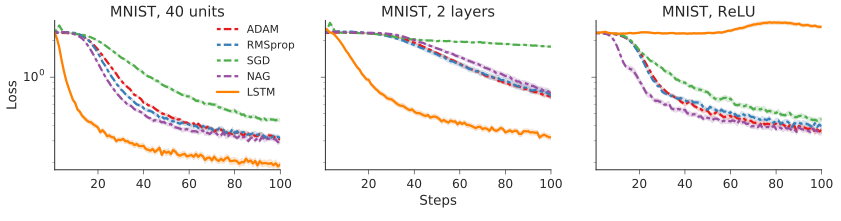
\includegraphics[scale=.8]{images/fig5.png}\\
        Trained on MLP with one hidden layer of 20 nodes. Examine how we can generalize to structure.
    \end{center}
}

\frame{
    \frametitle{Neural Art}
    \begin{center}
        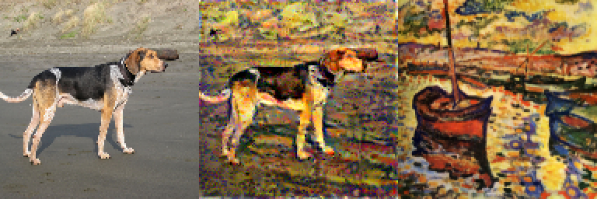
\includegraphics[scale=.8]{images/fig9-1.png}
        \quad
        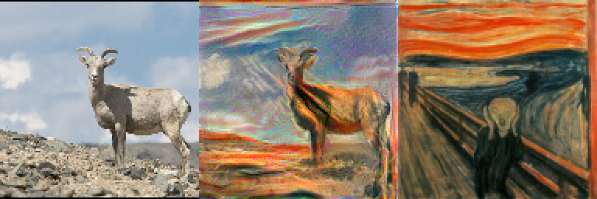
\includegraphics[scale=.8]{images/fig9-2.png}\\
        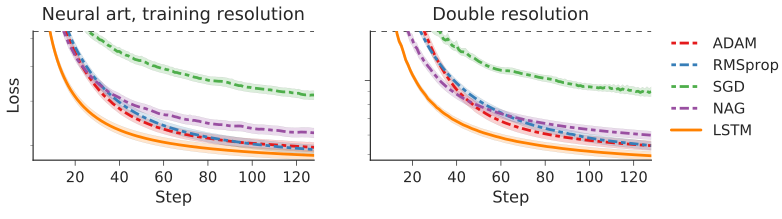
\includegraphics[scale=.8]{images/fig8.png}\\
        Optimize: $f(\theta) = \alpha\mathcal{L}_{content}(c,\theta) + \beta\mathcal{L}_{style}(s,\theta) + \gamma\mathcal{L}_{reg}(\theta)$
    \end{center}
}

\frame{
    \begin{center}
        \Huge{Questions/Discussion}
    \end{center}
}

\nocite{*} % Include everything in the .bib file.
\bibliographystyle{plainnat}
\bibliography{learning-to-learn}

% that's all, folks
\end{document}
